\documentclass[a4paper, 12pt]{article}

\usepackage[T2A]{fontenc}
\usepackage[utf8]{inputenc}

\usepackage[english, russian]{babel}

\usepackage{amsmath, amsfonts, amsthm, mathtools, amssymb}
\usepackage[left = 2cm, top=10mm, right=20mm, bottom=2cm, bindingoffset=0cm]{geometry}
\usepackage{setspace}
\setstretch{1.2}
%Рисунки
\usepackage{graphicx}
\usepackage{wrapfig }
\renewcommand{\arraystretch}{1.5}

\begin{document}
\begin{titlepage}
\centering
{\scshape\LARGE Московский физико-технический институт \par}
\vspace{3cm}
{\scshape\Large Лабораторная работа № 4.3.2(А) \par}
\vspace{1cm}
{\huge\bfseries Дифракция света на ультразвуковой волне в жидкости \par}
\vspace{0.5cm}
\vspace{1cm}
{\large\bfseries установка с вертикальной щелью \par}


\vfill
\begin{flushright}
{\large выполнила студентка группы Б03-303}\par
\vspace{0.3cm}
{\LARGE Мария Шишкарёва}
\end{flushright}
\vfill

\begin{figure}[h]
 \centering-
\includegraphics[width= 10 cm]{hv.png}
\end{figure}
% Bottom of the page
Долгопрудный, 2025 г.
\end{titlepage}





\large\section{Цель работы:}
изучение дифракции света на синусоидальной акустической решетке и наблюдение фазовой решетки методом темного поля.




\large\section{В работе используются:}
оптическая скамья, осветитель, два длиннофокусных объектива, кювета с жидкостью, кварцевый излучатель с микрометрическим винтом, генератор звуковой частоты, линза, вертикальная нить на рейтере, микроскоп.





\large\section{Теория:}
В данной работе исследовано явление \textit{дифракции}~-- отклонений в распространении света от законов геометрической оптики~-- на фазовой решётке, то есть в среде, осуществляющей периодическую модуляцию падающей волны света по фазе засчёт периодического изменения толщины и/или показателя преломления. В нашей работе рассмотрена дифракция на синусоидальной фазовой решётке в воде. При прохождении ультразвуковой волны через жидкость в ней возникают периодические неоднородности коэффициента преломления, и таким образом создается фазовая решетка, которую мы считаем неподвижной ввиду малости скорости звука относительно скорости света. Показатель преломления $n$ изменяется по закону:
\begin{equation*}
    n = n_0 (1 + m \cos \Omega x)
\end{equation*}
Здесь $\Omega = 2 \pi / \Lambda$~-- волновое число для ультразвуковой волны, $m$~-- глубина модуляции $ n $ $ (m \ll 1 $).
	
Положим фазу $ \varphi $ колебаний световой волны на передней стенке кюветы равной нулю, тогда на задней поверхности она равна:
\begin{equation*}
    \varphi  = k n L = \varphi_0 (1 + m \cos \Omega x)
\end{equation*}
Здесь $ L $ --- толщина жидкости в кювете, $ k = 2 \pi / \lambda $ --- волновое число для света.

После прохождения через кювету световое поле есть совокупность плоских волн, распространяющихся под углами $ \theta_m$, соответствующими максимумам в дифракции Фраунгофера:
\begin{equation}\label{eq1}	
    \Lambda \sin \theta_m = m \lambda
\end{equation}
Этот эффект проиллюстрирован на рисунке \ref{diff}.
\begin{figure}[h!]
    \centering	
    \includegraphics[width=0.3\textwidth]{Дифракция световых волн на акустической решетке.png}
    \caption{Дифракция световых волн на акустической решетке}
    \label{diff}
\end{figure}

Зная положение дифракционных максимумов, по формуле \eqref{eq1} легко определить длину ультразвуковой волны, учитывая малость $ \theta $: $ \sin \theta \approx \theta \approx l_m /F  $, где $ l_m $ --- расстояние от нулевого до последнего видимого максимума, $ F $ --- фокусное расстояние линзы. Тогда получим:
\begin{equation}
    \label{eq:1}
    \Lambda = m \lambda F/ l_m 
\end{equation}
Скорость ультразвуковых волн в жидкости, где $ \nu $ --- частота колебаний излучателя:
\begin{equation}
    v = \Lambda \nu 
\end{equation}
Стоит сформулировать качественный критерий, при выполнении
которого можно считать акустическую решётку чисто фазовой, т.\,е. рассматривать её как тонкий фазовый экран. Для нашей задачи условие
тонкого транспаранта можно записать в виде
\[
m\ll \frac{\Lambda}{L}\sqrt{\frac{\lambda}{L}}.
\]

В настоящей работе помимо дифракционного метода определения длины волны ультразвука используется способ получения видимого изображения акустической решётки~--— метод тёмного поля, основанный на устранении центрального дифракционного максимума с помощью специального экрана. Как нетрудно показать, в поле зрения микроскопа будут наблюдаться чередующиеся светлые и тёмные полосы, причём расстояние между тёмными полосами соответствует смещению в плоскости кюветы на $\Lambda/2$. Таким образом, должно наблюдаться характерное для метода тёмного поля удвоение числа деталей рассматриваемой структуры.






\large\section{Схема установки:}
Схема установки приведена на рисунке 2. Источник света Л через светофильтр Ф и конденсор К освещает вертикальную щель $ S $, находящуюся в фокусе объектива $ O_1 $. После объектива параллельный световой пучок проходит через кювету С перпендикулярно акустической решетке, и дифракционная картина собирается в фокальной плоскости объектива $ O_2 $ , наблюдается при помощи микроскопа М.

    Предварительную настройку установки произведем в соответствии с инструкцией с зеленым фильтром, далее в работе используется красный.
    
    	\begin{figure}[h!]
    	\centering	
    	\includegraphics[width=15 cm]{stand.png}
    	\caption{Схема для наблюдения дифракции на акустической решетке}
    	\label{shema1}
    \end{figure}


\begin{figure}[h!]
    	\centering	
    	\includegraphics[width=15 cm]{Снимок экрана 2025-02-22 103933.png}
    	\caption{Схема для наблюдения дифракции методом тёмного поля}
    	\label{shema1}
    \end{figure}





\large\section{Результаты измерений:}
\subsection{Определение скорости ультразвука по дифракционной картине}
\begin{table}[]
\begin{tabular}{|l|l|l|l|l|}
\hline
   & $\nu_{1}$ = 1.19 МГц & $\nu_{2}$ = 3.97 МГц & $\nu_{3}$ = 1.59МГц & $\nu_{4}$ = 1.83 МГц \\ \hline
m  & $x_{m}$, мкм         & $x_{m}$, мкм         & $x_{m}$, мкм        & $x_{m}$, мкм         \\ \hline
-3 & 1188                 &                      &                     &                      \\ \hline
-2 & 1044                 & 1336                 & 1120                & 1192                 \\ \hline
-1 & 892                  & 828                  & 916                 & 928                  \\ \hline
0  & 752                  & 712                  & 696                 & 696                  \\ \hline
1  & 584                  & 256                  & 625                 & 464                  \\ \hline
2  & 440                  & -520                 & 284                 & 240                  \\ \hline
3  & 268                  &                      &                     &                      \\ \hline
\end{tabular}
\end{table}
\newpage



\subsection{Определение скорости ультразвука методом тёмного поля}
Опытным путём определили цену деления окулярной шкалы: 1 дел = $\frac{1}{6}$ мм
\par
\begin{table}[h]
\begin{tabular}{|l|l|l|l|l|}
\hline
$\nu_{1}$, МГц & 1.17 & 1.6 & 1.83 & 1.48 \\ \hline
$x_{1}$, дел   & 101  & 72  & 62   & 90   \\ \hline
$x_{1}$, дел   & 11   & 21  & 0    & 0    \\ \hline
N              & 24   & 22  & 37   & 28   \\ \hline
\end{tabular}
\end{table}






\large\section{обработка результатов:}
\subsection{Определение скорости ультразвука по дифракционной картине}
\par
По результатам измерений построим графики зависимоти $x_{m}$(m) для всех частот
\par
По коэффициенту наклона для каждой частоты найдём $\Lambda$ по формуле (2)
\par
По формуле (3) находим значение скорости ультразвука.
\par
Результаты заносим в таблицу

\begin{table}[h]
\begin{tabular}{|l|l|l|l|l|}
\hline
$\nu$, МГц & $\Lambda$, мм & $\sigma_{\Lambda}$, мм & v, м/с & $\sigma_{v}$, м/с \\ \hline
1.19       & 1.32         & 0.17                  & 1571.6 & 198.4             \\ \hline
3.97       & 0.43         & 0.05                  & 1732.6 & 218.3             \\ \hline
1.59       & 0.97         & 0.12                  & 1540.6 & 194.4             \\ \hline
1.83       & 0.85         & 0.17                  & 1557.0 & 305.1             \\ \hline
\end{tabular}
\end{table}
\newpage

\begin{figure}[h]
\centering
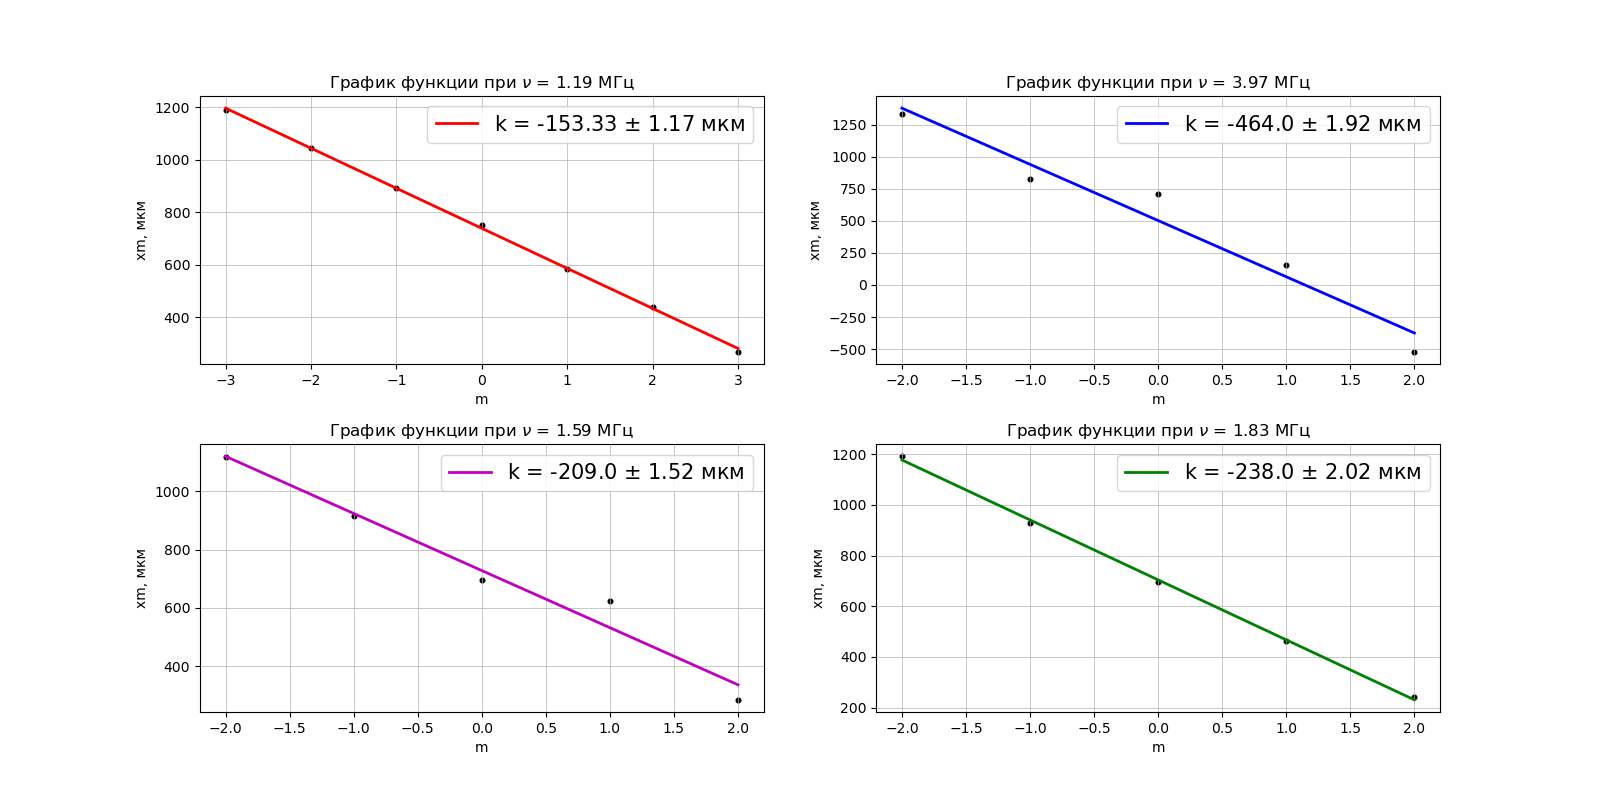
\includegraphics[width= 18 cm]{График зависимости xm(m) при разных частотах.png}
\end{figure}



\subsection{Определение скорости ультразвука методом тёмного поля}
\par
Рассчитаем длину УЗ-волны с учётом удвоением числа деталей, наблюдаемых методом тёмного поля.
\par
Определим скорость УЗ в воде
\par
Результаты занесём в таблицу
\begin{table}[h]
\begin{tabular}{|l|l|l|l|l|}
\hline
$\nu$, МГц & $\Lambda$, мм & $\sigma_{\Lambda}$, мм & v, м/с & $\sigma_{v}$, м/с \\ \hline
1.17       & 1.250        & 0.007                 & 1462.5 & 10.3              \\ \hline
1.6        & 0.772        & 0.008                 & 1236.3 & 12.7              \\ \hline
1.83       & 0.559        & 0.004                 & 1022.2 & 8.7               \\ \hline
1.43       & 1.071        & 0.006                 & 1532.1 & 10.0              \\ \hline
\end{tabular}
\end{table}





\large\section{Вывод:}
В работе изучена дифракция света на акустической решетки, рассчитаны длина волны ультразвука и скорость его распространения в воде. Решетка наблюдалась методом
темного поля.





\end{document}
